\documentclass{article}
\usepackage{graphicx} % for images

\title{DS 740 Midterm Executive Summary}
\author{Sean Murphy}
\date{July 2024}

\begin{document}

\maketitle

\section{Introduction}

One of the major challenges when shopping for a vehicle is to purchase one with as many desired 
features as possible within one's price range. Often, prospective vehicle owners must narrow down 
their wish list of features to afford a vehicle.  Developing a model that could predict a vehicle's 
retail price based on its features would be extremely useful.  It is this exact task that this 
modeling process is designed to address.  The data used to develop this model was a 2004 data set 
containing fifteen features of 429 vehicles and their retail price.  The goal was to create a model 
that accurately predicts a vehicle's retail price based on its features.  The two model types that I 
considered in this analysis were robust regression and elastic net, with varying tuning parameter 
values.

\section{Data Cleaning}

% introduce missingness plots
\begin{figure}
    \centering
    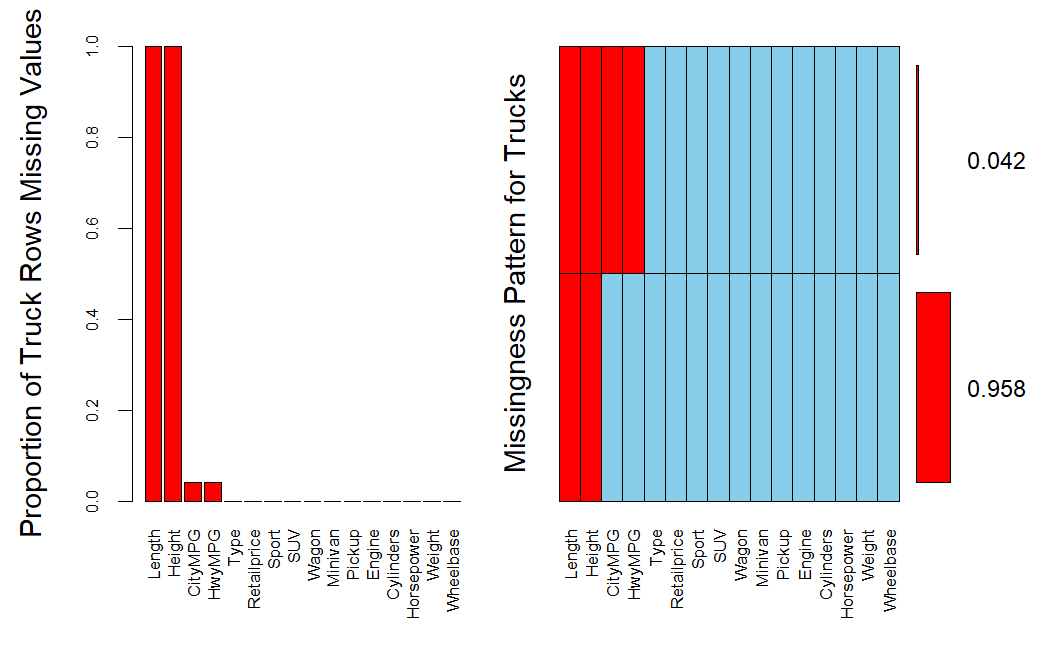
\includegraphics[scale = 0.6]{truck_missingness.png}
    \caption{Missingness pattern for truck entries in the data set reveals all trucks are missing 
    length and height measurements.}
    \label{fig:truck_missingness}
\end{figure}

A few major data-cleaning tasks preceded the model-fitting process. First, missing values needed to 
be addressed. Overall, about $9.58\%$ of the entries contained missing values. The height and length 
variables contained the highest proportion of nulls, with just over $6\%$ each. Upon further examination, 
I found that every truck in the data set was missing values for these variables, as can be seen in 
Figure~\ref{fig:truck_missingness}.  To address these missing values, I first removed the height and 
length columns so that predictions for trucks would not disproportionately suffer due to their consistent 
lack of data.  Then, I removed the rows containing missing values in other fields, so that not all trucks 
would be removed from the data set.  

% introduce correlation plot
\begin{figure}
    \centering
    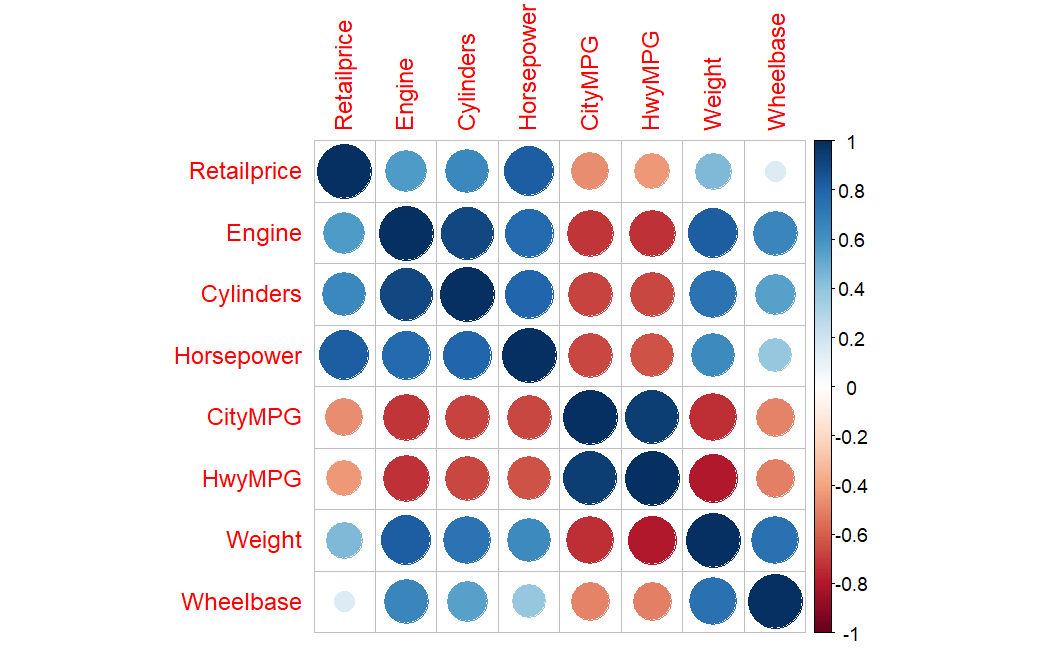
\includegraphics[scale = 0.8]{correlation_plot.png}
    \caption{Correlation plot revealing some multicollinearity amongst the numeric predictors.}
    \label{fig:corrplot}
\end{figure}

Next, I examined the correlation plot of the numeric predictors in Figure~\ref{fig:corrplot}.  Although 
some predictors were highly correlated, I decided to advance without removing any.  Since the elastic 
net model can shrink some coefficients to zero, this would likely help address redundant predictors. 

I then fitted a multiple linear regression model on all the predictors to examine the residual plots.  
The plots revealed heteroscedasticity of the residuals and deviation from normality.  They also revealed 
some significant outliers.  I decided to keep these outliers in the data set since methods like ridge 
regression are resistant to them.  The violated assumptions for multiple linear regression could also be 
overcome by the more complex models considered in this analysis.

Finally, I examined the distribution of the response, retail price.  I found that it was right-skewed, 
so I performed a log transformation and removed the original response from the data set.  Then, I 
proceeded to consider tuning parameters.  

\section{Tuning Parameters}

The tuning parameters to consider for this modeling process were $\lambda$ and $\alpha$ values for the 
elastic net model. 
 $\alpha$ values range from $0$ (ridge regression) to $1$ (LASSO).  Thus, I chose to consider $\alpha$ 
 values $0$, $0.2$, $0.4$, $0.6$, $0.8$, and $1$.  
 
 $\lambda$ is a tuning parameter that controls coefficient shrinkage. I began by considering a wide, 
 exponential range of values with a greater density towards the lower values.  Since the initial 
 optimal $\lambda$ value was at the smaller end of this range, I reduced the range to include values 
 between $0.001$ and $1$, incremented by $0.001$.  This smaller range would reduce the run time of my 
 code and ignore irrelevant $\lambda$ values.  I then proceeded to fit the models.  

\section{Best Model and Interpretation}

% introduce the heat plot
\begin{figure}
    \centering
    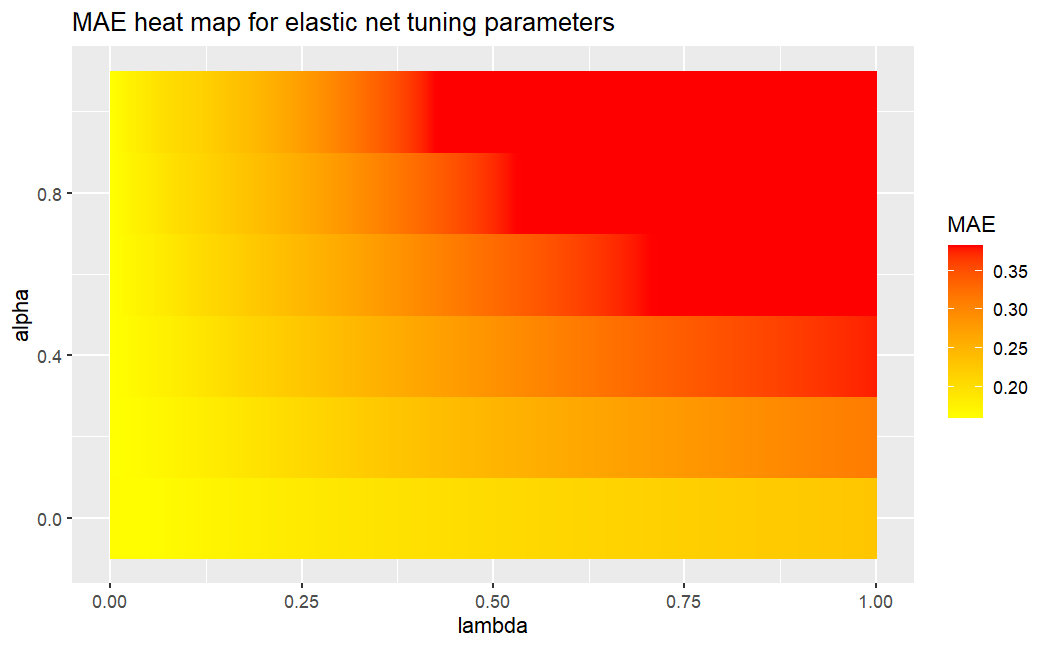
\includegraphics[scale = 0.6]{heat_plot.png}
    \caption{MAE values tend to shrink for smaller tuning parameter values in the elastic net models.}
    \label{fig:heat_plot}
\end{figure}

I used 10-fold cross-validation to fit the ridge regression and elastic net models on the data.  For 
ridge regression, I considered default combinations of weights (Tukey, Huber, and Hampel) and intercepts.  
For the elastic nets, I considered every combination of $\alpha$ and $\lambda$ that I introduced above.  
As one can see in Figure~\ref{fig:heat_plot}, the MAE for elastic net models tends to shrink for smaller 
values of each tuning parameter. 
 After fitting the models, I found that the elastic net model with $\alpha = 0.2$ and $\lambda = 0.003$ 
 had the lowest cross-validated MAE of $0.1608$.  I then fit this model to the entire data set.

% introduce the violin plots
% pickups
\begin{figure}
    \centering
    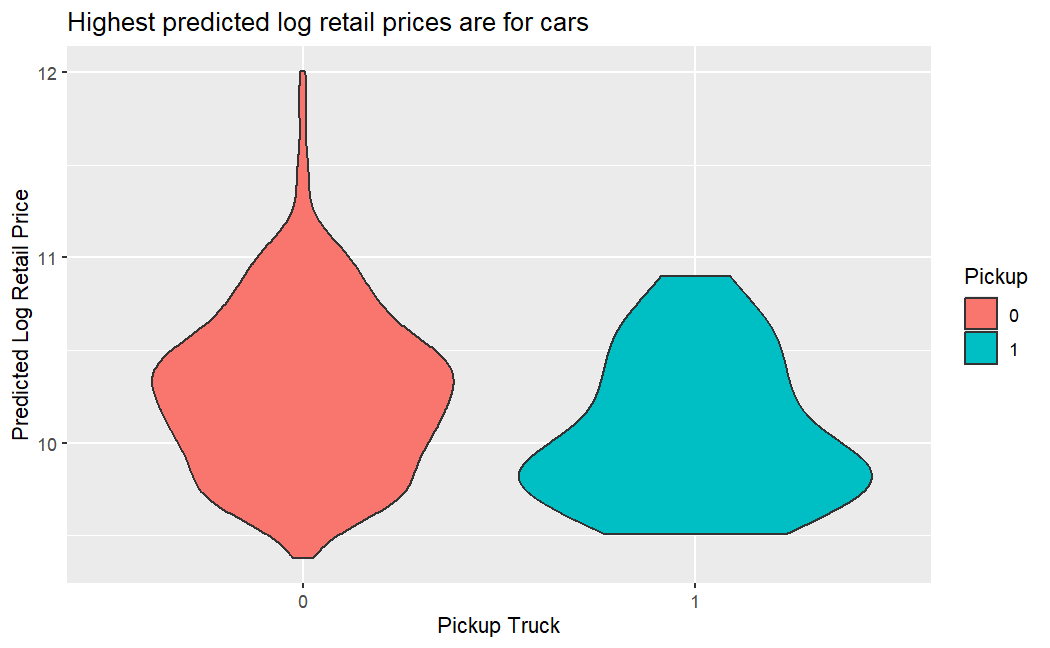
\includegraphics[scale = 0.6]{pickups_vs_preds.png}
    \caption{Violin plots of the predicted response versus whether or not a vehicle is a pickup truck.}
    \label{fig:pickup_violin}
\end{figure}
% SUVs
\begin{figure}
    \centering
    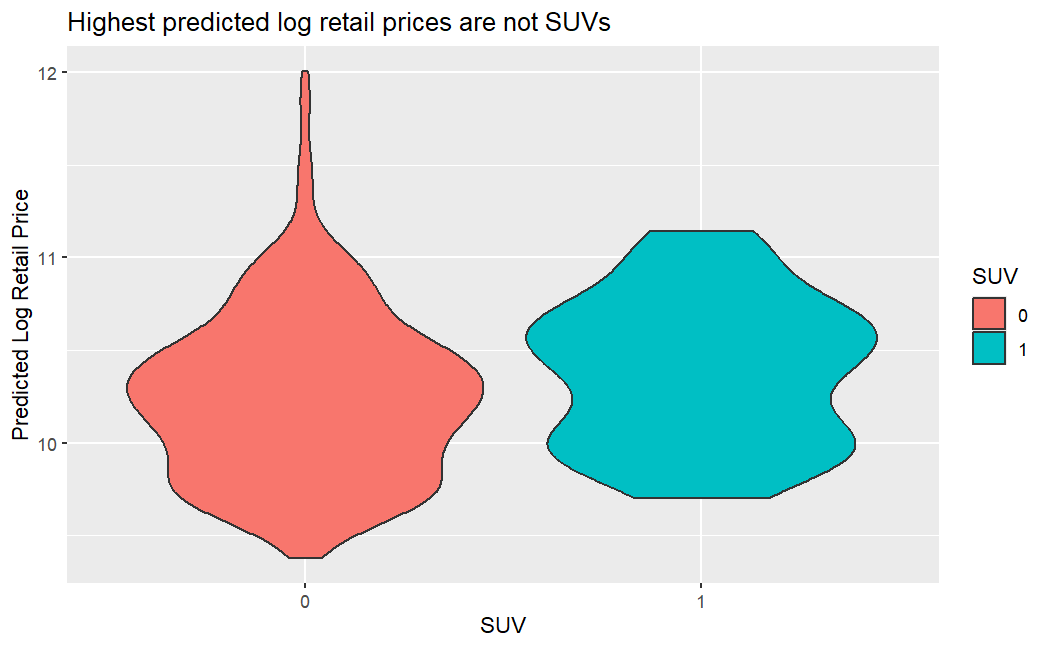
\includegraphics[scale = 0.6]{suvs_vs_preds.png}
    \caption{Violin plots of the predicted response versus whether or not a vehicle is an SUV.}
    \label{fig:suv_violin}
\end{figure}

After fitting the final model, I examined the variable importance measures for each predictor.  I found 
that the two most important predictors in the model were the indicators for pickup trucks and SUVs 
respectively.  I then examined the relationship between each of these variables and the predicted log 
of the retail price, as in Figures ~\ref{fig:pickup_violin} and ~\ref{fig:suv_violin}.  For both of 
these predictors, the predicted log retail prices were highest for vehicles that did not possess the 
trait.  In other words, the highest predicted log retail prices were for vehicles that were neither 
pickup trucks nor SUVs.  This relationship with the predicted response is unsurprising, since the most 
expensive vehicles tend to be luxury or sport vehicles, categories which pickup trucks and SUVs do not 
tend to fall into.  

However, it is somewhat surprising that these were the two most important predictors of the response.  
I would initially have thought that the indicator for sports cars, as well as the horsepower measurement, 
would be more influential.  

\section{Accuracy of Model Fitting Process}

Finally, I performed 5-fold cross-validation on the entire modeling process to assess its accuracy.  I 
found that the outer cross-validated MAE (after exponentiating the response and predictions) was about 
$\$5,742.55$ in context.  This is the best estimate of the MAE for the best model selected iteratively 
in repeated analyses among the models considered here for this data set.  This is a fairly low average 
error rate, especially since retail prices in the data set range all the way from $\$10,280$ to 
$\$192,465$.  Thus, while not perfect, this model-fitting process and its resulting model certainly can 
be used by customers looking to purchase a vehicle to gain insight into the price of their ideal vehicle.

Though this model is useful, it certainly could be improved. Some specific fields might be helpful to 
include in addition to those already in the data set. For one, the vehicle brand would likely improve 
prediction accuracy, as specific brands tend to vary consistently in their pricing. Another field could 
be an indicator for additional vehicle features, such as convertibles or sunroofs.  If possible, these 
data should be included in subsequent analyses.  

Overall, this analysis has developed a reasonably accurate model to be used for predicting vehicle 
retail prices among vehicles in 2004 (and perhaps later).  Between the robust regression and elastic 
net models considered in this analysis, the elastic net model performs best on this data set.  

\end{document}